\chapter{Спектры простых сигналов}

\section{Цель работы}
Получить представление о свойствах спектров.

\section{Постановка задачи}
В командном окне MATLAB и в среде Simulink промоделировать следующие тестовые сигналы:
\begin{itemize}
\item Полигармонический сигнал
\item Прямоугольный импульсный сигнал
\item Треугольный импульсный сигнал
\end{itemize}
Получить спектров этих сигналов.

\section{Теоретическая часть}
\begin{itemize}
\item Полигармонический сигнал y(t)=$\sum\limits_{n=0}^{N-1} cos (nt)$ \newline
\item Прямоугольный импульсный сигнал y(t)=$\prod(t,Ti)$ \newline
\item Треугольный импульсный сигнал y(t)=$\Delta(t,Ti)$
\end{itemize}
\section{Ход работы}

\subsection{Код Matlab}
\begin{lstlisting}
close all;
clear all;
x = 0:0.01:4*pi;
f0 = 5;
%исходный сигнал
%for n=1:length(x)
%  y(n) = cos(2*pi*f0*n*x(n));
%end;
for n=1:length(x)
  if mod(n,20) < 10
      y(n) = 0;
  else
      y(n) = 1;
  end;
end;
figure
plot(x(1:200),y(1:200))
axis([-0.5 2.5 -0.5 1.5])
y = conv(y,y);
for n=1:length(x)
    y(n) = y(n)/n;
end;
figure
plot(x(1:200),y(1:200))
grid
%спектр исходного сигнала
figure
spectrum = fft(y,512);
norm_spectrum = spectrum.*conj(spectrum)/512;
f=100*(0:255)/512;
plot(f, norm_spectrum(1:256))
axis([0 max(f) 0 1000])
grid

clear all;

t = 0:00.1:4*pi;
N = 100;
y = 0;

% Полигармонический сигнал
y = sin(pi*t)+sin(3*pi*t)+sin(pi*0.3*t);
plot(t,y)
grid

figure
spectrum = fft(y,512);
norm_spectrum = spectrum.*conj(spectrum)/512;
f=100*(0:255)/512;
plot(f, norm_spectrum(1:256))
axis([0 max(f) 0 10])
grid

% Треугольный сигнал
figure
y2 = conv(square(t,20),square(t,20));
plot(t(1:100),y2(1:100));
grid

figure
spectrum = fft(y2,512);
norm_spectrum = spectrum.*conj(spectrum)/512;
f2=100*(0:255)/512;
plot(f2, norm_spectrum(1:256)/1000)
axis([0 max(f2) 0 50])
grid

\end{lstlisting}

\begin{figure}[H]
   \includegraphics[scale=0.7]{lab5/poly.png}
   \caption{Полигармонический сигнал}
\end{figure}

\begin{figure}[H]
   \includegraphics[scale=0.7]{lab5/poly_spectro.png}
   \caption{Спектр gолигармонического сигнала}
\end{figure}

\begin{figure}[H]
   \includegraphics[scale=0.7]{lab5/rect.png}
   \caption{Прямоугольный сигнал}
\end{figure}

\begin{figure}[H]
   \includegraphics[scale=0.7]{lab5/rect_spectro.png}
   \caption{Спектр прямоугольного сигнала}
\end{figure}

\begin{figure}[H]
   \includegraphics[scale=0.7]{lab5/triangle.png}
   \caption{Треугольный сигнал}
\end{figure}

\begin{figure}[H]
   \includegraphics[scale=0.7]{lab5/triangle_spectro.png}
   \caption{Спектр треугольного сигнала}
\end{figure}

\subsection{Simulink}

В ходе моделирования сигналов в Simulink были собраны следующие схемы и получены соответствующие графики:

\begin{figure}[H]
\centering
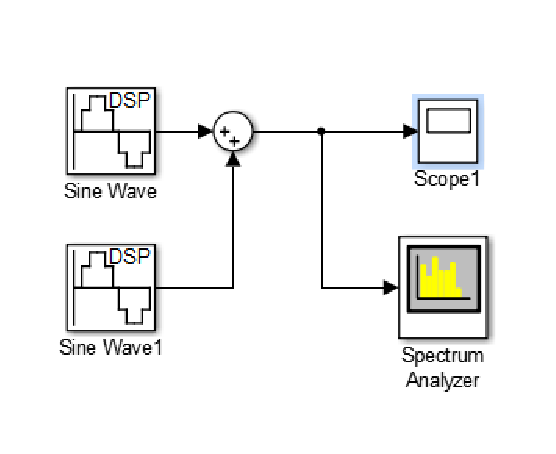
\includegraphics[width=10cm]{lab5/1_simulink} 
\caption{Полигармонический сигнал (Simulink)} 
\end{figure}

\begin{figure}[H]
\centering
\includegraphics[width=10cm]{lab5/lab5_1_simulink} 
\caption{Полигармонический сигнал} 
\end{figure}

\begin{figure}[H]
\centering
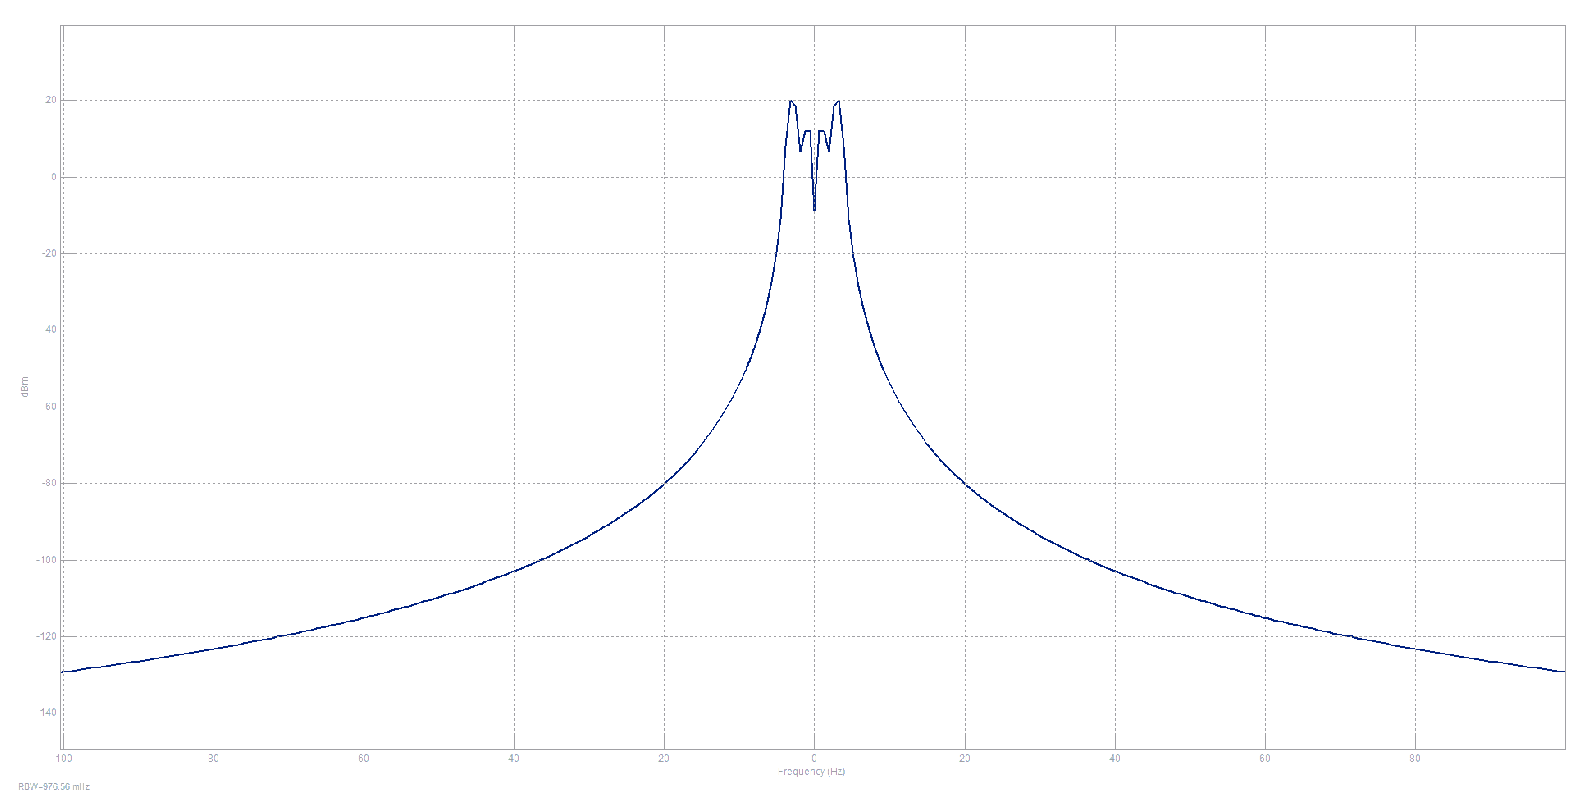
\includegraphics[width=10cm]{lab5/lab5_2_simulink}
\caption{Спектр полигармонического сигнала} 
\end{figure}

\begin{figure}[H]
\centering
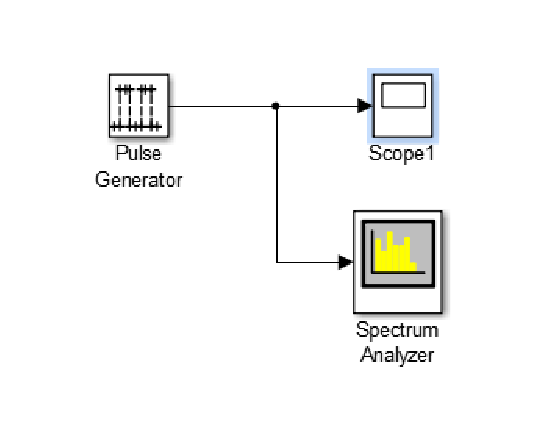
\includegraphics[width=10cm]{lab5/3_simulink} 
\caption{Прямоугольный импульсный сигнал (Simulink)} 
\end{figure}

\begin{figure}[H]
\centering
\includegraphics[width=10cm]{lab5/lab5_3_simulink} 
\caption{Прямоугольный импульсный сигнал} 
\end{figure}

\begin{figure}[H]
\centering
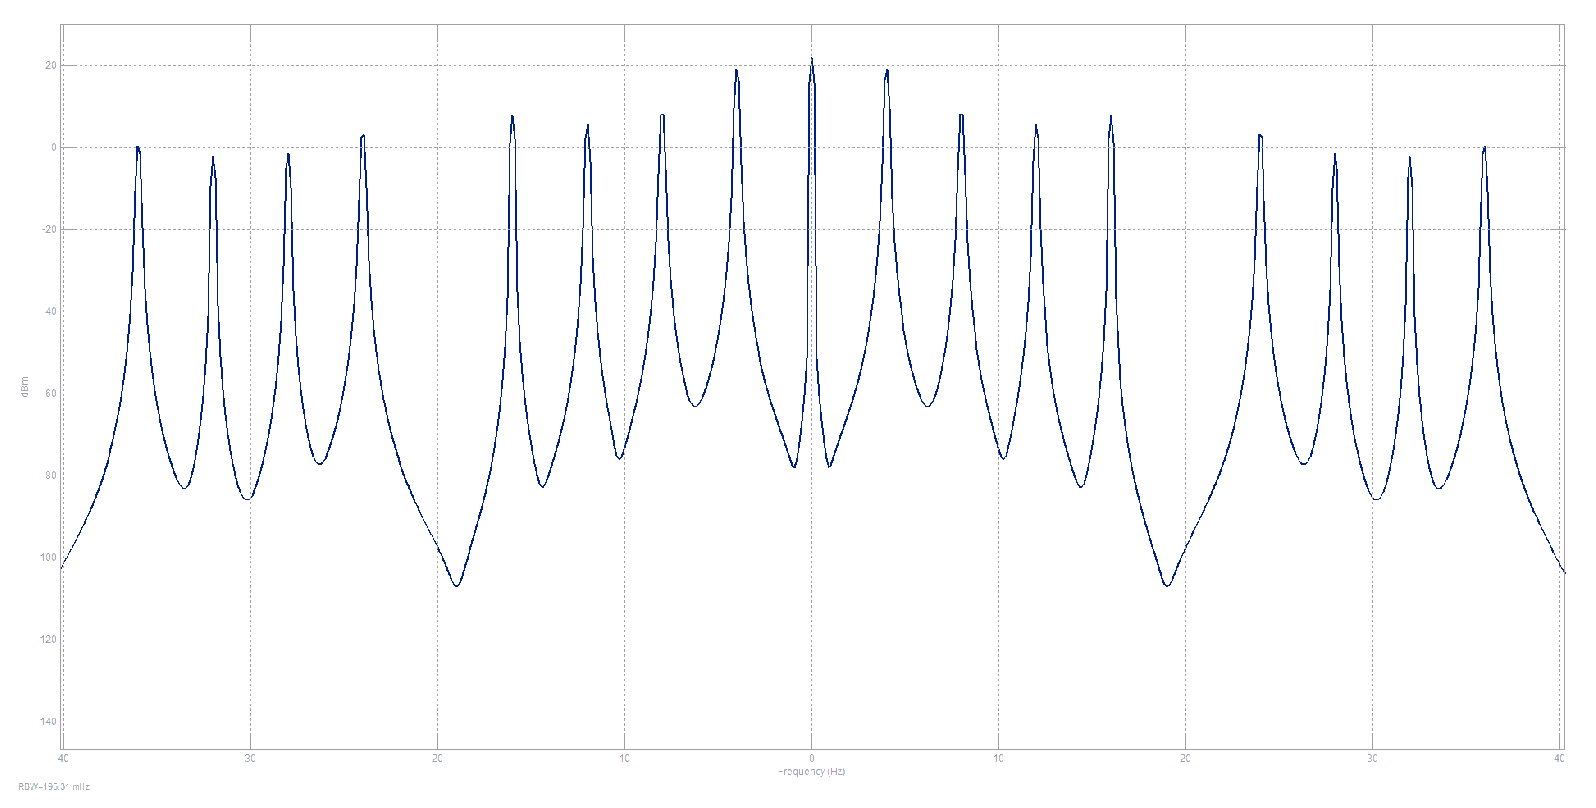
\includegraphics[width=10cm]{lab5/lab5_4_simulink}
\caption{Спектр прямоугольного сигнала} 
\end{figure}

\begin{figure}[H]
\centering
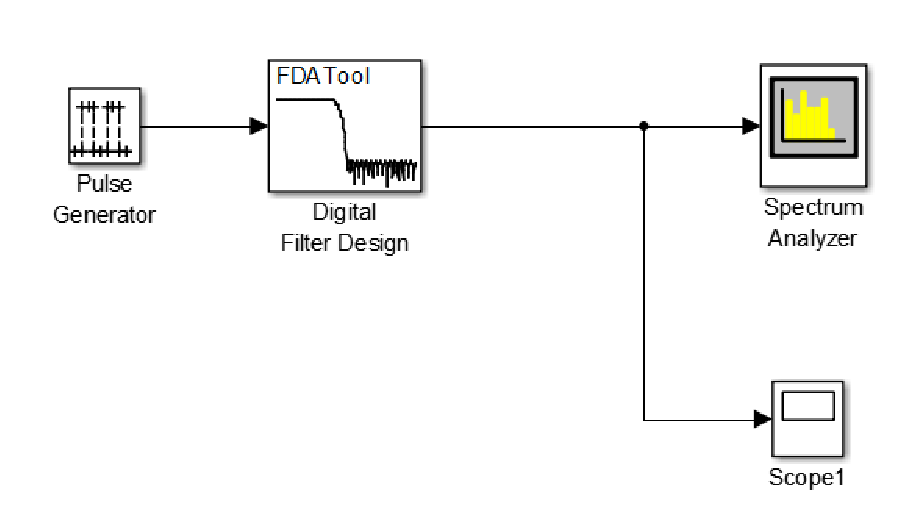
\includegraphics[width=10cm]{lab5/4_simulink} 
\caption{Треугольный импульсный сигнал (Simulink)} 
\end{figure}

\begin{figure}[H]
\centering
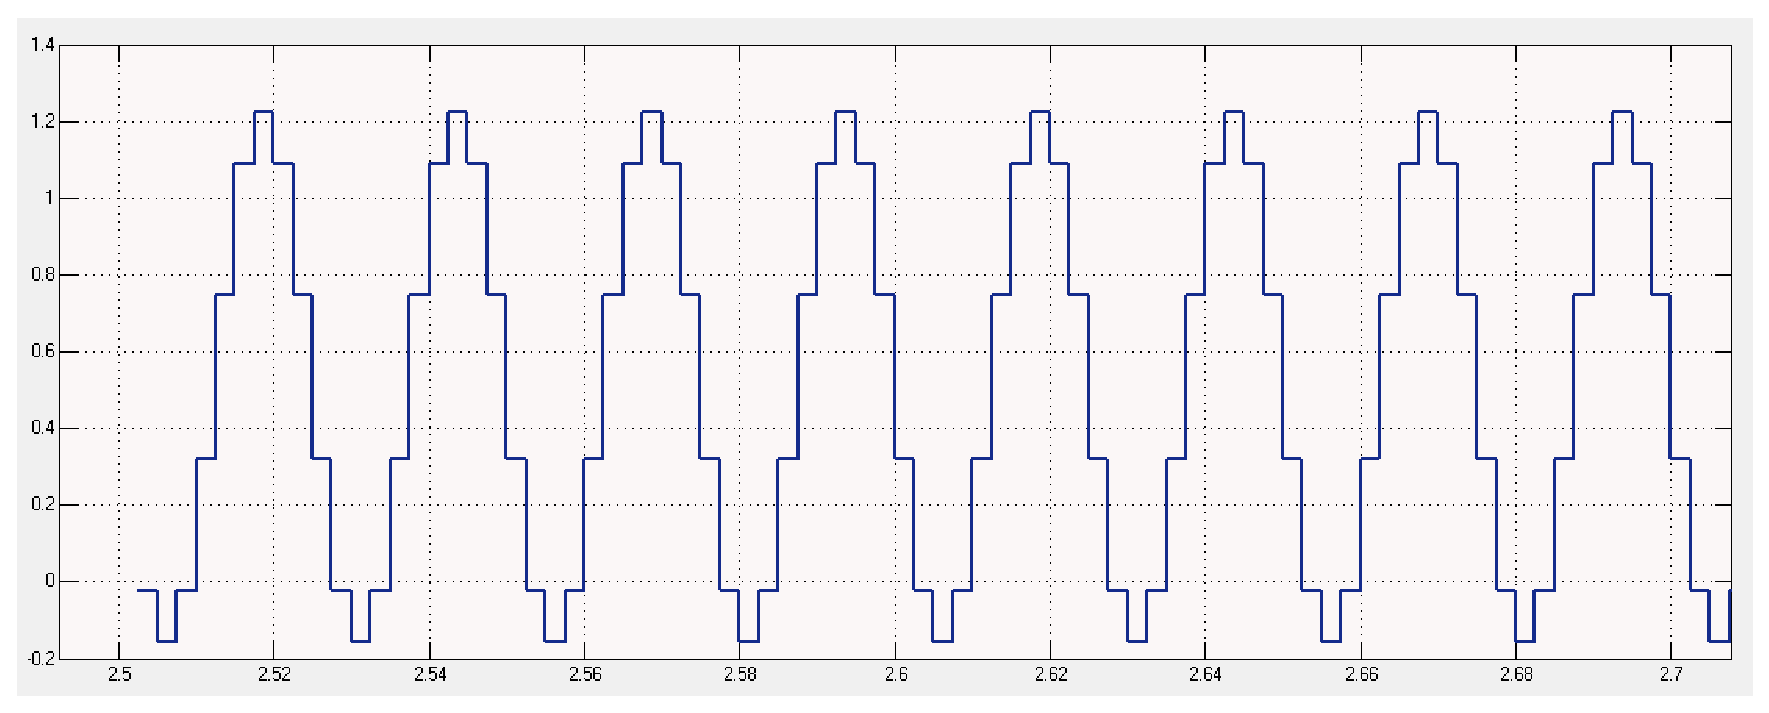
\includegraphics[width=10cm]{lab5/lab5_5_simulink} 
\caption{Треугольный импульсный сигнал} 
\end{figure}

\begin{figure}[H]
\centering
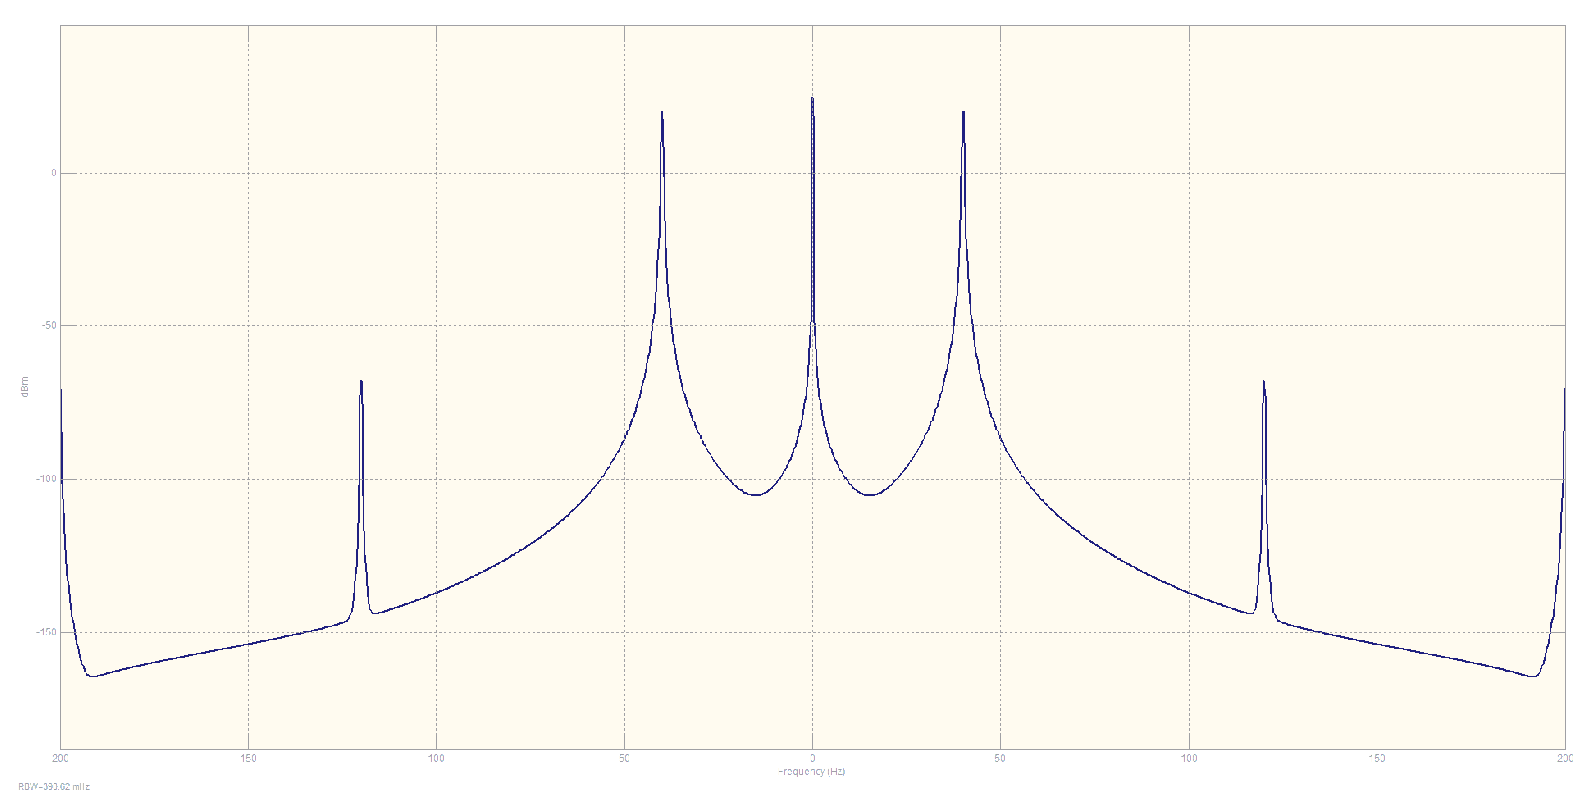
\includegraphics[width=10cm]{lab5/lab5_6_simulink}
\caption{Спектр треугольного сигнала} 
\end{figure}

\section{Выводы}
В результате проделанной работы было проведено моделирование в среде MatLAB и Simulink полигармонического, прямоугольного и треугольного импульсных сигналаов, а также получены их спектры. В Simulink для получения генератора треугольного сигнала используется генератор прямоугольных импульсов каскадно с фильтром с прямоугольным окном. Это обоснуется тем, что свертка двух прямоугольных импульсов в результате дает треугольный.